% =====================================================================
%  PLA DE TREBALL (PT) -- Concurs LE-403/729 (UPC)
%  Version 2 (16/11/2026), built on PT_skeleton.tex. American English, aligned with the
%  HAP (three research lines, HAP numbering of publications [J], [R], [C], [D]).
%  General context on the UPC, the EEBE and the subjects adapted from the PT of
%  J. Calafell and the Professor Agregat project, rewritten in English.
%  Personal data: ONLY name and surname (base 3.5).
%  Before submitting: uncomment \finaltrue to hide the marks.
%  Output file name: Monteiro_Carlos_PT.pdf
% =====================================================================
\documentclass[11pt]{article}
\usepackage{lector}
\usepackage{pgfgantt}
\usetikzlibrary{arrows.meta,positioning}
\newcommand{\sectionbreak}{\clearpage}
%\finaltrue
\setupheader{PT}

\title{\textbf{Pla de Treball}\\[2pt]\large Work Plan}
\author{\Large \CandName}
\date{}

\begin{document}
\maketitle
\thispagestyle{plain}
\vspace{0.5cm}
\begin{center}\postdata\end{center}

%\vspace{0.8cm}
%\noindent\textbf{Summary.}
This work plan outlines the research, teaching, supervision, and funding objectives to be pursued over the six-year duration of the Lector contract for position LE-403/729, starting in September 2027.
The research programme is structured around three interconnected lines aligned with the position's research profile: (i) the physics of supercritical turbulent flows; (ii) the causal analysis and prediction of extreme events in multiphysics turbulence; and (iii) high-performance computing for compressible, real-fluid turbulent flows. Together, these lines aim to advance the understanding, prediction, and mitigation of complex thermofluid phenomena in supercritical fluid systems, with particular emphasis on pseudo-boiling effects relevant to propulsion technologies and supercritical power cycles. The principal scientific contributions will include the development and consolidation of a generalizable Lagrangian framework for identifying the causal mechanisms underlying extreme turbulent events, particularly intermittent thermal loading, and new physical insights into the onset and mechanisms of heat-transfer deterioration.
In parallel, the teaching plan builds on my current experience in Thermodynamics and Heat Transfer and Fluid Engineering, proposes contributions to the master's course in Computational Fluid Mechanics, and establishes connections between student theses and the proposed research activities. The supervision strategy envisions two doctoral theses supported by competitive predoctoral grants. Finally, the funding strategy establishes a progressive transition from collaborative research within the GReCEF group towards scientific independence, through the leadership of a nationally funded research project and the preparation of an ERC Starting Grant proposal towards the end of the contract.

\newpage
\tableofcontents

% =====================================================================
\section{Research plan}\label{sec:research}

\subsection{Background and motivation}\label{sec:background}

%\paragraph{Supercritical fluids in engineering.} 
Fluids operated above their critical pressure are central to several energy and propulsion technologies. 
In supercritical CO$_2$ (sCO$_2$) thermodynamic cycle technology, the high density of the working fluid near the critical point reduces the necessary size of the turbomachinery by about one order of magnitude with respect to steam Rankine cycles and can raise the thermal efficiency by up to five percentage points~\cite{Ahn2015}. 

Liquid-rocket engines cool their thrust chambers regeneratively with
propellants (hydrogen, methane or kerosene) flowing at supercritical pressure through
narrow channels next to the hot wall~\cite{Pizzarelli2018,Nasuti2021}, and inject them into
combustion chambers at pressures above the critical pressure of the
propellants~\cite{JofreUrzay2021,Bellan2020}. Supercritical fluids are also used in
refrigeration and heat pumps~\cite{Nieuwenhuyse2023}, in supercritical-water reactors and
oxidation processes, and in chemical extraction~\cite{Brunner2010,Yoo2013}.

\paragraph{National and European priorities in space propulsion.} Spain invests directly in
space transportation: in 2024 the Ministry of Science, Innovation and Universities, through
the CDTI and within the PERTE Aeroespacial, allocated \texteuro{}40.5 million to the development
phase of the first Spanish small-satellite launcher~\cite{CDTI2024}. At the European level,
ESA's Future Launchers Preparatory Programme (FLPP) seeks, through THRUST!~2, to demonstrate
staged-combustion engines for high-thrust liquid propulsion~\cite{ESA2026}, whose thrust
chambers are regeneratively cooled and fed by propellants at supercritical
pressure~\cite{Pizzarelli2018}. These programs address engine design and testing; this plan
contributes the fundamental understanding of transcritical heat transfer, mixing and
near-wall thermal protection on which the models used in that design rely. Spanish companies
developing liquid-rocket engines, such as PLD Space and the Barcelona-based Pangea Aerospace,
which designed a regeneratively cooled demonstrator with real-fluid models of supercritical
oxygen and methane~\cite{Esnault2021}, are prospective partners for transfer and industrial
doctorates.

\paragraph{The pseudo-boiling region.} Above the critical pressure there is no
liquid--vapor phase change. However, an isobaric change of temperature drives the fluid
from a liquid-like to a gas-like state across a narrow region around the pseudo-boiling
temperature $T_{pb}$, where the specific heat peaks and density, viscosity and thermal
conductivity drop steeply~\cite{Banuti2015}. For CO$_2$ at 8~MPa
(figure~\ref{fig:background}a), density decreases sixfold and viscosity fivefold between
$0.91\,T_{pb}$ and $1.17\,T_{pb}$, while the specific heat at $T_{pb}$ is 15 to 25 times
larger than at the ends of this interval. This behavior is the source of both the
advantages and the difficulties of these fluids. The large heat capacity and density
enable compact, efficient heat exchange~\cite{Ahn2015}. In heated channels, however, the
same property variations can cause heat-transfer deterioration (HTD): a local drop of the
heat-transfer coefficient that produces a peak of wall temperature, typically when the wall
temperature exceeds $T_{pb}$ while the bulk remains below it~\cite{Urbano2013}. HTD is still
not fully understood and is hardly predictable, which is critical in rocket engines and
nuclear reactors, where a wrong estimate of the wall temperature can lead to failure of the
component~\cite{Pizzarelli2018}. The thermodynamics of this region remains an active field:
recent reviews identify open questions on the structure of the supercritical state itself
and report that the velocity and temperature transformations developed for variable-property
flows succeed only for moderate density ratios~\cite{Li2025}.

\paragraph{Pseudo-boiling and turbulence.} Direct numerical simulation (DNS) has
established that the property variations of pseudo-boiling modulate near-wall turbulence
and heat transfer in heated pipes, annuli and channels~\cite{Bae2005,Peeters2016,Nemati2016,Kawai2019,Guo2022,Wan2025}.
A distinctive feature is the very dissimilar behavior of the two walls of a differentially
heated channel: the cold wall is bathed by a dense, liquid-like fluid and the hot wall by a
light, gas-like fluid, so that the turbulence and the thermal structures differ markedly
between them~\cite{Ma2018,Guo2022,ElMansy2025}. Even for water, whose properties vary far less, recent
DNS shows that the friction coefficient changes by $-39\,\%$ to $+32\,\%$ with respect to
constant-property flow, and that empirical correlations deviate by up to 26~\% from the
DNS~\cite{Modesti2026}. Pseudo-boiling flows are much more extreme, and their predictive
description is correspondingly weaker.

\paragraph{The SCRAMBLE context and my contribution.} The ERC project SCRAMBLE, in which I
carried out my PhD, exploits pseudo-boiling to achieve turbulence in microdevices. Near the
pseudo-boiling line the kinematic viscosity drops sharply, which raises the bulk Reynolds
number of a microchannel from about $170$ to above $2000$ for the same geometry and bulk
velocity~\cite{Hurtan2025}. In addition, the strong density gradients generate baroclinic
torque, which destabilizes the flow and promotes the transition to
turbulence~\cite{Bernades2023,Bernades2025}. Within this project, the group has developed the
numerical methods~\cite{BernadesKEEP2023} and the open-source solver RHEA [J1], and I have
contributed resolution and minimal-domain standards for DNS of transcritical wall turbulence
[J5, J6], characterized the flow regimes of microconfined flows [J3, J4, J7], and shown that
buoyancy reorganizes the secondary flows of square ducts and redistributes momentum and heat
[J2, R1, C1].

\begin{figure}[t]
\centering
\begin{minipage}[c]{0.40\textwidth}\centering
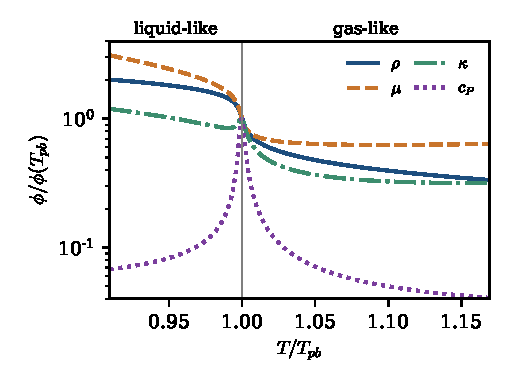
\includegraphics[width=\textwidth]{images/co2_pseudoboiling.pdf}\\[-2pt]
{\small (a)}
\end{minipage}\hfill
\begin{minipage}[c]{0.58\textwidth}\centering
\resizebox{\linewidth}{!}{\begin{tikzpicture}[font=\scriptsize, x=1cm, y=1cm,
  arr/.style={-{Stealth[length=1.5mm]}, line width=0.6pt}]
% ---- thrust chamber and nozzle (upper half), wall with coolant passage
\def\inner{(0,1.05) -- (1.4,1.05) .. controls (2.0,1.05) and (2.1,0.55) .. (2.5,0.55)
           .. controls (2.9,0.55) and (3.4,1.0) .. (4.3,1.45)}
\def\outer{(0,1.40) -- (1.4,1.40) .. controls (2.0,1.40) and (2.1,0.90) .. (2.5,0.90)
           .. controls (2.9,0.90) and (3.4,1.35) .. (4.3,1.80)}
\fill[orange!12] (0,0) -- \inner -- (4.3,0) -- cycle;
\draw[line width=0.9pt, black!70] \inner;
\draw[line width=0.9pt, black!70] \outer;
\draw[black!40] (0,0) -- (4.3,0);
\node[orange!70!black, align=center] at (0.85,0.55) {hot combustion\\ gas};
\draw[arr, orange!80!black] (0.25,0.15) -- (1.45,0.15);
% coolant path inside the wall (from nozzle exit to injector)
\draw[arr, UPCAccent, line width=0.9pt] (4.15,1.62) .. controls (3.4,1.18) and (2.9,0.72) .. (2.5,0.72)
      .. controls (2.1,0.72) and (2.0,1.22) .. (1.4,1.22) -- (0.15,1.22);
\node[UPCAccent, align=center, anchor=south] at (3.55,1.72) {coolant in\\ ($p>p_c$, $T<T_{pb}$)};
\node[UPCAccent, anchor=south] at (0.55,1.42) {to injector};
\draw[arr, red!70!black] (2.5,0.15) -- (2.5,0.50);
\node[red!70!black, align=center] at (2.5,-0.18) {throat: peak $q_w$};
\draw[dashed, black!50] (1.8,1.55) -- (1.8,0.85) node[pos=0,above] {A};
% ---- cross-section A-A
\begin{scope}[shift={(4.9,0.05)}]
  \fill[black!12] (0,0) rectangle (2.55,1.55);
  \foreach \x in {0.2,1.05,1.9} {
    \shade[top color=UPCAccent!35, bottom color=red!45] (\x,0.45) rectangle ++(0.45,0.85);
    \draw[black!60] (\x,0.45) rectangle ++(0.45,0.85);
    \draw[dashed, black!70] (\x,0.72) -- ++(0.45,0);
  }
  \foreach \x in {0.35,0.85,1.35,1.85,2.35} \draw[arr, red!70!black] (\x,-0.35) -- (\x,0.02);
  \node[red!70!black] at (1.27,-0.52) {$q_w$ (one-sided heating)};
  \node[align=left, anchor=west] at (2.65,1.2) {liquid-like core};
  \node[align=left, anchor=west] at (2.65,0.85) {\textbf{- -} $T=T_{pb}$};
  \node[align=left, anchor=west] at (2.65,0.5) {gas-like near wall};
  \draw[black!50] (2.35,1.1) -- (2.65,1.2); \draw[black!50] (2.35,0.72) -- (2.65,0.85); \draw[black!50] (2.35,0.55) -- (2.65,0.5);
  \node[anchor=south] at (1.27,1.58) {section A--A};
\end{scope}
\end{tikzpicture}}\\[-2pt]
{\small (b)}
\end{minipage}
\caption{(a) Thermophysical properties of CO$_2$ at 8~MPa across the pseudo-boiling
temperature $T_{pb}=307.8$~K, normalized by their values at $T_{pb}$ (computed with
CoolProp~\cite{CoolProp2014}). (b) Regenerative cooling of a liquid-rocket thrust chamber
(schematic): the propellant flows at supercritical pressure through rectangular channels in the
chamber wall, heated on the hot-gas side only; near the heated wall it crosses $T_{pb}$ and becomes
gas-like, which can trigger heat-transfer deterioration~\cite{Pizzarelli2018,Nasuti2021,Urbano2013}.}
\label{fig:background}
\end{figure}

\paragraph{Open challenges.} Five gaps limit the prediction of these flows:
\begin{enumerate}[label=(\roman*)]
  \item \textbf{Reynolds number.} Most DNS of pseudo-boiling wall turbulence are performed at
  Reynolds numbers one to two orders of magnitude below those of the
  applications~\cite{Li2025}, so the scaling of friction and heat transfer with Reynolds
  number is uncertain.
  \item \textbf{Complex geometries.} Cooling passages and compact heat exchangers have
  rectangular cross-sections, where corners and secondary flows redistribute momentum and
  heat. Apart from our own work [R1, C1], I am not aware of DNS of pseudo-boiling flows in
  square ducts.
  \item \textbf{Developing flows and HTD.} HTD develops along heated channels, but DNS of
  spatially developing pseudo-boiling flows is limited to round tubes at low Reynolds
  numbers~\cite{Bae2005,Zhao2021}. Regenerative cooling channels, in addition, are heated on
  one side only, which changes the onset of deterioration~\cite{Nasuti2021}.
  \item \textbf{Free shear flows.} High-fidelity studies of transcritical jets and mixing
  layers exist~\cite{Ries2017,SharanBellan2021,PobladorIbanez2026}, and recent simulations of
  oxygen--hydrogen mixing layers at rocket-engine conditions show that the thermodynamic model
  changes the growth rate and the small-scale mixing, most strongly near the critical
  pressure~\cite{Cavalieri2026}. Turbulent pseudo-boiling rates have also been quantified with
  large-eddy simulations of transcritical oxygen--methane flames~\cite{Cavalieri2025}, where the
  pseudo-boiling transition occurs below the grid scale. Single-fluid jets, in which the jet and its
  environment are the same substance (nitrogen or CO$_2$) on opposite sides of the
  pseudo-boiling temperature, have shown that pseudo-boiling strongly stratifies the jet near the
  critical pressure and enhances its shear-layer instability and decay~\cite{Lapenna2019,Ream2025}; these studies analyze statistics and
  spectra, not the interfaces. Therefore, the effect of
  pseudo-boiling on the turbulent/non-turbulent and turbulent/turbulent interfaces that
  control entrainment, characterized in detail for constant-property
  flows~\cite{Silva2018,Alves2025}, remains unexplored. These interfaces govern mixing in
  injection~\cite{JofreUrzay2021} and the coolant layer in film cooling.
  \TODO{add one film-cooling reference at supercritical pressure}
  \item \textbf{Extreme events.} Design limits are set by the largest local excursions of
  wall heat flux and wall temperature, not by their averages. These rare events are not
  captured by mean correlations, and their causes in pseudo-boiling flows are unknown
  (Section~\ref{sec:lines}, Line~2).
\end{enumerate}

\subsection{Research lines, open questions and objectives}\label{sec:lines}
The plan addresses these gaps through three lines, which correspond to the three research
lines of the call. Each line states its open questions (Q) and the objectives (O) that
answer them.

\subsubsection*{Line 1 -- Physics of supercritical turbulent flows by direct numerical
simulation (profile line a)}
High-fidelity data are scarce in the regimes that matter for the applications: at higher
Reynolds numbers in channels and square ducts, in spatially developing ducts with HTD, and in
free shear flows across pseudo-boiling. This line generates and analyzes such data.
\begin{itemize}
  \item[\textbf{Q1.1}] How do pseudo-boiling and the asymmetry between liquid-like and
  gas-like walls change friction and heat transfer as the Reynolds number increases, and
  how do corners and secondary flows modify them in square ducts?
  \item[\textbf{Q1.2}] Which mechanisms trigger HTD and its recovery in a spatially developing
  square duct, and how do they depend on the heat-flux-to-mass-flux ratio and on one-sided
  heating?
  \item[\textbf{Q1.3}] How does pseudo-boiling modify the entrainment across the interfaces
  of a jet or mixing layer?
\end{itemize}
\textbf{Objectives.}
\begin{itemize}
  \item[\textbf{O1.}] Generate two open DNS databases with real-fluid
  thermodynamics~\cite{PengRobinson1976,Chung1988}: (a) fully developed differentially heated
  channel and square duct at friction Reynolds numbers above those of our current
  databases; and (b) a spatially developing, heated square duct that reaches and recovers
  from HTD.
  \item[\textbf{O2.}] Derive predictive tools from these data: extend the integral
  transformations recently developed for variable-property flows~\cite{Modesti2026} to
  pseudo-boiling conditions, and train compact neural networks for wall-normal profiles,
  in collaboration with Prof.\ X.\ Yang (Penn State).
  \item[\textbf{O3.}] (Phase~2, exploratory) Characterize the turbulent/non-turbulent and
  turbulent/turbulent interfaces of a temporal mixing layer and a temporal planar jet of a
  single fluid, in which a liquid-like stream meets a gas-like stream of the same substance at
  supercritical pressure. This single-component, single-phase configuration isolates
  pseudo-boiling from species diffusion, phase separation and combustion, as in the classical
  experiments and simulations of cryogenic nitrogen injected into warm nitrogen at
  supercritical pressure~\cite{Mayer2003,Muller2016,Lapenna2019}, and it is resolved with the
  real-fluid DNS framework of Line~1. The interface detection and entrainment analysis will be
  developed with the group of Prof.\ C.\ B.\ da Silva (Instituto Superior T\'ecnico).
\end{itemize}

\subsubsection*{Line 2 -- Causality and extreme events in multiphysics turbulence (profile
line b)}
In regenerative cooling, extreme positive and negative excursions of the wall heat flux
impose local thermal loads that may damage the wall. Extreme wall events in turbulence have
been characterized by conditional averaging and space--time
analysis~\cite{Guerrero2020,Hack2021,Zhang2023}, and their predictability has been
examined~\cite{Blonigan2019}; our group has also proposed conditional POD to predict extreme
events from time signals~\cite{Martin2025}. Conditional averages, however, reveal what
accompanies an event, not what causes it. Information-theoretic measures such as transfer
entropy~\cite{Schreiber2000}, the Liang--Kleeman information flow~\cite{Liang2005} and the
decomposition of causality into synergistic, unique and redundant
components~\cite{MartinezSanchez2024} quantify cause and effect, and have been applied to
wall turbulence~\cite{LozanoDuran2020,Massaro2023,Zhang2026}. These estimators usually
assume stationary, long time series, whereas extreme events are rare and non-stationary.
Ensemble estimators for non-stationary signals exist in other fields~\cite{Wollstadt2014},
and Lagrangian information-theoretic analyses have recently been applied to
flows~\cite{Jiang2027}. In the 2026 CTR Summer Program, I combined event-conditioned
Eulerian fields, Lagrangian trajectories and event-anchored transfer entropy to identify the
precursor sequence of extreme wall-heat-flux events in four DNS of transcritical channel
flow [R3], which provides the starting point of this line.
\begin{itemize}
  \item[\textbf{Q2.1}] Are current causality estimators reliable for rare, non-stationary
  events, and how many independent events do they require?
  \item[\textbf{Q2.2}] Which processes, and in which order, cause extreme wall-heat-flux
  events in pseudo-boiling flows, and how do they differ from a low-pressure reference?
  \item[\textbf{Q2.3}] Do the identified precursors improve the prediction of these events?
  \item[\textbf{Q2.4}] Does the framework transfer to other multiphysics problems?
\end{itemize}
\textbf{Objectives.}
\begin{itemize}
  \item[\textbf{O4.}] Assess current estimators on synthetic and canonical signals with known
  causal structure, and formalize an event-anchored Lagrangian information-theoretic
  framework, released as open-source code.
  \item[\textbf{O5.}] Apply it to the Line~1 databases to identify the causes of extreme
  wall-heat-flux events and to test precursor-based prediction against conditional
  statistics and conditional POD~\cite{Martin2025}.
  \item[\textbf{O6.}] Transfer it to two further problems: the aggregation and settling of
  microplastics with biogenic particles in ocean
  turbulence~\cite{Rahmani2022,Pizzi2024,Pizzi2026}, with the University of British Columbia
  and, locally, with the Institut de Ci\`encies del Mar (ICM-CSIC), a partner of our group in
  experiments on biofilm growth on microplastics~\cite{Pizzi2025}; and extreme wall heat flux
  in compressible boundary layers, starting with the stay at the Universit\`a del Salento.
\end{itemize}

\subsubsection*{Line 3 -- High-performance computing for compressible, real-fluid
turbulence (profile line c)}
The DNS of Lines 1 and 2 require GPU-resident solvers. RHEA-X, the distributed GPU version of
RHEA for which I was responsible, combines MPI and OpenACC and shows near-ideal scaling on
large GPU systems [J1]. GPU-accelerated solvers are now widespread in turbulence
research~\cite{Roccon2026}, and state-of-the-art compressible solvers such as STREAmS have been
rewritten to support several GPU back-ends~\cite{Bernardini2021,Bernardini2023}. Europe's first exascale
system, JUPITER, entered operation in 2025. In real-fluid simulations, a large part of the cost
comes from the equation of state and the transport coefficients; low-rank surrogates reduce
it and suit GPU execution [R4]. Quantum algorithms for flow problems are an emerging,
long-term option that I will follow but not pursue in this plan~\cite{Bharadwaj2023}.
\begin{itemize}
  \item[\textbf{Q3.1}] Which parts of a real-fluid compressible solver limit performance on
  current GPU architectures, and how much can kernel optimization and surrogates reduce them?
  \item[\textbf{Q3.2}] How can large ensembles of Lagrangian trajectories be tracked in situ
  without limiting the scalability required by Line~2?
\end{itemize}
\textbf{Objectives.}
\begin{itemize}
  \item[\textbf{O7.}] Profile and optimize the kernels of RHEA-X, integrate the GPU surrogates
  of real-fluid properties, and publish reproducible benchmarks of cost and accuracy versus
  problem size and GPU count.
  \item[\textbf{O8.}] Implement in-situ Lagrangian tracking and statistics, and port the
  solver to the architectures of the EuroHPC systems.
\end{itemize}

\subsection{Growth of the research lines and long-term direction}\label{sec:growth}
The three lines are designed to grow from canonical problems towards engineering conditions,
and each step is supported by an external group that has selected, adopted or co-developed
the work.
\begin{itemize}
  \item \textbf{Line 1} starts from databases that are already used outside the group: they
  contribute to the BLASTNet machine-learning dataset coordinated by Prof.\ M.\ Ihme
  (Stanford University) [D1], and Prof.\ X.\ Yang (Penn State) uses them to train neural
  networks. The square-duct results will be presented at EFDC3 (2027). The line moves from
  fully developed to developing ducts, and only then, in Phase~2, to free shear flows.
  Supercritical flows remain the main focus of the plan.
  \item \textbf{Line 2} was selected through the competitive call of the 2026 CTR Summer
  Program and will be presented at THMT-27 (2027). Its formalization draws on non-stationary
  transfer entropy, developed with A.\ Chandra (CTR), and on the information-theoretic
  causality developed by Prof.\ A.\ Lozano-Dur\'an and \'A.\ Mart\'inez-S\'anchez
  (Caltech, MIT). It is then tested by other groups on their own problems: ocean turbulence
  at UBC (stay in summer 2027, before the contract) and compressible boundary layers at the
  Universit\`a del Salento (first half of 2028). A prospective stay in the United States
  (2029--30), at Stanford University or Caltech, would consolidate the compressible
  extension.
  \item \textbf{Line 3} builds on a published solver [J1], two BSC hackathons and six
  peer-reviewed supercomputing allocations. Its development serves Lines 1 and 2 and will
  be strengthened through the BSC hackathons and bachelor's and master's projects in
  scientific computing at the EEBE.
\end{itemize}

\paragraph{Long-term direction.} With mature databases (Line~1), a validated causal framework
(Line~2) and an efficient solver (Line~3), Phase~2 targets a central engineering problem of
the field: to explain, predict and ultimately prevent HTD in its applications, from
regenerative cooling channels to the heat exchangers of sCO$_2$
cycles~\cite{Pizzarelli2018,Ahn2015}. Beyond the contract, the same capabilities lead
naturally to high-speed aerothermodynamics, where extreme wall heat fluxes, large property
variations and thermochemical effects coexist~\cite{Urzay2018,DiRenzoUrzay2021,Passiatore2022}.
The stays at the Universit\`a del Salento and in the United States prepare this extension,
in line with the department's priority on compressible flows.

\subsection{Work plan and timeline}\label{sec:workplan}
The plan covers six years, from September 2027 to August 2033, with Year~1 corresponding to
the academic year 2027--28. Scientifically, it is divided into two phases, consistent with the
intermediate evaluation of the contract: \textbf{Phase~1 (years 1--3), foundations}:
databases, causal framework and optimized solver; and \textbf{Phase~2 (years 4--6),
prediction}: HTD prediction and transfer to other flows. In parallel, the Lector position
provides the framework to build an independent research program within GReCEF, in three
stages:
\begin{itemize}
  \item \textbf{Establishment (Y1--Y2, 2027--29):} integration into GReCEF, initial funding,
  continued publication as first author, first doctoral recruitment, the Salento stay and the first proposal as principal
  investigator.
  \item \textbf{Development (Y3--Y4, 2029--31):} execution of the first independent project,
  if funded; a small team of two doctoral students and master's students; the stay in the
  United States.
  \item \textbf{Consolidation (Y5--Y6, 2031--33):} research leadership, the ERC Starting Grant
  proposal, follow-up funding, and research accreditation towards stabilization.
\end{itemize}
The work is organized in five work packages (WPs).

\paragraph{WP1 -- Supercritical turbulence databases (Line~1; O1--O3; Y1--Y6).} Carried out
mainly by doctoral student~1, under my supervision and co-supervision within GReCEF.
\emph{Tasks:} T1.1 fully developed channel and square duct at higher Reynolds numbers
(Y1--Y3); T1.2 spatially developing heated square duct with HTD (Y2--Y4); T1.3 transformations
and compact neural networks for friction and heat transfer, with Penn State (Y3--Y5); T1.4
exploratory single-fluid temporal mixing layer and planar jet across pseudo-boiling (Y5--Y6).
\emph{Outcomes:} two open databases, 3--4 journal articles and doctoral thesis~1.

\paragraph{WP2 -- Causality and extreme events (Line~2; O4--O6; Y1--Y6).} Led by me.
\emph{Tasks:} T2.1 assessment of estimators and formalization of the Lagrangian framework,
with open-source code (Y1--Y2); T2.2 extreme wall-heat-flux events in the WP1 databases and
precursor-based prediction (Y2--Y4); T2.3 microplastics in ocean turbulence, from the results
of the UBC stay, with ICM-CSIC (Y1--Y3); T2.4 compressible boundary layers, during the
Salento stay and the prospective US stay (Y1--Y3); T2.5 HTD prediction combining the
framework with the WP1 developing-duct database (Y4--Y6).
\emph{Outcomes:} 3--4 journal articles, an open-source causality code and joint articles with
the host groups.

\paragraph{WP3 -- Solver performance and exascale readiness (Line~3; O7, O8; Y1--Y6).}
\emph{Tasks:} T3.1 profiling and kernel optimization of RHEA-X, prepared and tested in BSC
hackathons (Y1--Y3); T3.2 integration of GPU surrogates of real-fluid properties [R4] (Y1--Y2);
T3.3 in-situ Lagrangian tracking for WP2 (Y2--Y4); T3.4 porting and benchmarks on EuroHPC
systems (Y3--Y6). Bachelor's and master's theses at the EEBE contribute to T3.1--T3.3;
doctoral student~2 (Phase~2) can take T3.3--T3.4 or T2.5.
\emph{Outcomes:} versioned open-source releases, 1--2 articles and the computing allocations
required by WP1 and WP2.

\paragraph{WP4 -- Resources, group building and management (Y1--Y6).} Applications for
funding and computing time (Section~\ref{sec:resources}); recruitment of doctoral students
1 (Y2) and 2 (Y3--Y4); Year-3 self-assessment; research accreditation (Y5--Y6).

\paragraph{WP5 -- Mobility, collaborations and dissemination (Y1--Y6).} Stays and
collaborations (Section~\ref{sec:mobility}) and dissemination
(Section~\ref{sec:dissemination}).

\begin{center}\small
\begin{tabularx}{\textwidth}{@{}p{0.8cm}p{1.35cm}X@{}}
\toprule
\textbf{Mil.} & \textbf{Year} & \textbf{Milestone} \\
\midrule
M1 & Y1 & First version of the causality framework; publication of the square-duct and CTR work [R1, R3]; Salento stay; predoctoral applications for doctoral student~1. \\
M2 & Y2 & First proposal as principal investigator (\emph{Generaci\'on de Conocimiento}, Tipo~A) submitted; doctoral student~1 recruited; open-source causality code released; application for the US stay. \\
M3 & Y3 & First open database (O1a); optimized solver release; US stay; start of the independent project, if funded; Year-3 self-assessment. \\
M4 & Y4 & Developing-duct HTD database (O1b); doctoral student~2 recruited. \\
M5 & Y5 & First HTD predictions; ERC Starting Grant proposal in preparation; application for research accreditation. \\
M6 & Y6 & ERC Starting Grant proposal submitted; follow-up national proposal; defense of doctoral thesis~1. \\
M7 & Y6 & Exploratory free-shear results; consolidated independent line on HTD and extreme events. \\
\bottomrule
\end{tabularx}
\end{center}

\begin{figure}[H]
\centering
\definecolor{GLineA}{HTML}{2F5D8A}%
\definecolor{GLineB}{HTML}{C8742B}%
\definecolor{GLineC}{HTML}{3C8D6E}%
\definecolor{GCross}{HTML}{8C96A0}%
\definecolor{GFund}{HTML}{6B4C9A}%
\definecolor{GDec}{HTML}{C0392B}%
\begin{ganttchart}[
    hgrid={*1{black!10}},
    vgrid={*3{black!10, dashed}, *1{black!35}},
    x unit=0.48cm, y unit title=0.5cm, y unit chart=0.47cm,
    time slot format=simple,
    canvas/.append style={draw=black!35, line width=0.4pt},
    title/.append style={draw=black!35, fill=MSBlue!12},
    title label font=\scriptsize\bfseries\color{MSBlue},
    title height=1,
    bar height=0.5, bar top shift=0.25,
    bar/.append style={draw=none, rounded corners=1.5pt},
    bar label font=\scriptsize,
    bar label node/.append style={align=right},
    milestone/.append style={fill=GFund, draw=none},
    milestone label font=\scriptsize,
    milestone height=0.5, milestone top shift=0.25
  ]{1}{24}
  \gantttitle{Establishment}{8}\gantttitle{Development}{8}\gantttitle{Consolidation}{8}\\
  \gantttitle{Y1 27--28}{4}\gantttitle{Y2 28--29}{4}\gantttitle{Y3 29--30}{4}\gantttitle{Y4 30--31}{4}\gantttitle{Y5 31--32}{4}\gantttitle{Y6 32--33}{4}\\
  \ganttbar[bar/.append style={fill=GLineA}]{T1.1 Developed channel/duct}{1}{12}\\
  \ganttbar[bar/.append style={fill=GLineA}]{T1.2 Developing duct (HTD)}{5}{16}\\
  \ganttbar[bar/.append style={fill=GLineA!60}]{T1.3 Transformations, NN}{9}{20}\\
  \ganttbar[bar/.append style={fill=GLineA!40}]{T1.4 Free shear (expl.)}{17}{24}\\
  \ganttbar[bar/.append style={fill=GLineB}]{T2.1 Causal framework}{1}{8}\\
  \ganttbar[bar/.append style={fill=GLineB}]{T2.2 Extreme heat flux}{5}{16}\\
  \ganttbar[bar/.append style={fill=GLineB!60}]{T2.3 Ocean (UBC, ICM)}{1}{12}\\
  \ganttbar[bar/.append style={fill=GLineB!60}]{T2.4 Compressible BL}{2}{12}\\
  \ganttbar[bar/.append style={fill=GLineB!40}]{T2.5 HTD prediction}{13}{24}\\
  \ganttbar[bar/.append style={fill=GLineC}]{T3.1--T3.2 Kernels, surrogates}{1}{12}\\
  \ganttbar[bar/.append style={fill=GLineC!60}]{T3.3--T3.4 Lagrangian, EuroHPC}{5}{24}\ganttnewline[black!60]
  \ganttbar[bar/.append style={fill=GFund!35}]{ALECTORS, GReCEF projects}{1}{6}\\
  \ganttbar[bar/.append style={fill=GFund!35}]{PID Tipo A: prep., subm., decision}{2}{4}%
  \ganttmilestone[inline]{}{6}%
  \ganttmilestone[inline, milestone/.append style={fill=GDec}]{}{9}\\
  \ganttbar[bar/.append style={fill=GFund}]{PID project (if funded)}{10}{21}%
  \ganttbar[inline, bar/.append style={fill=GFund!25, draw=GFund, dashed}]{}{22}{24}\\
  \ganttbar[bar/.append style={fill=GFund!35}]{ERC StG: prep., submission}{17}{20}%
  \ganttmilestone[inline]{}{21}\\
  \ganttmilestone{Follow-up national proposal}{22}\\
  \ganttbar[bar/.append style={fill=GCross}]{Stays (Salento, US)}{3}{3}%
  \ganttbar[inline, bar/.append style={fill=GCross!40, draw=GCross, dashed}]{}{10}{11}\\
  \ganttbar[bar/.append style={fill=GFund!35}]{PhD 1: funding, thesis, defense}{1}{4}%
  \ganttbar[inline, bar/.append style={fill=GLineA!70}]{}{6}{22}%
  \ganttmilestone[inline, milestone/.append style={fill=MSBlue}]{}{23}\\
  \ganttbar[bar/.append style={fill=GFund!35}]{PhD 2 (FPI, if funded)}{10}{12}%
  \ganttbar[inline, bar/.append style={fill=GLineA!70}]{}{13}{24}\\
  \ganttmilestone[milestone/.append style={fill=GDec}]{Year-3 self-assessment}{12}\\
  \ganttbar[bar/.append style={fill=GFund!35}]{Research accreditation (AQU)}{17}{20}%
  \ganttmilestone[inline]{}{21}
\end{ganttchart}
\caption{Timeline by quarters (Y1 = 2027--28). Upper block: scientific tasks
(\textcolor{GLineA}{$\blacksquare$}~Line~1, \textcolor{GLineB}{$\blacksquare$}~Line~2,
\textcolor{GLineC}{$\blacksquare$}~Line~3). Lower block: light purple bars, proposal preparation
or applications; purple diamonds, submissions; red diamonds, expected funding decision and
evaluation; solid bars, execution and doctoral theses; dashed bars, conditional or optional
periods. The UBC stay (summer 2027) precedes Y1. All dates after Y1 are indicative and depend
on future calls and on successful evaluation.}
\end{figure}

\subsection{Resources, funding strategy and risk management}\label{sec:resources}
\paragraph{Starting point.} The ERC Starting Grant SCRAMBLE, which currently funds my
postdoctoral position, and the infrastructure of GReCEF cover the first months of WP1--WP3.

\paragraph{Independent output before the first project.} Until a project as principal
investigator starts (2029 at the earliest), the research does not depend on new funding: it
builds on the existing databases, the RHEA-X solver and yearly competitive computing
allocations. During Y1--Y2 I will keep publishing as first and corresponding author in the
lines I lead: the square-duct and causality manuscripts [R1--R3], the causal framework
(T2.1) and the joint work of the UBC and Salento stays, with a target of at least two journal
articles per year. This record of independent output is the basis of the first proposal as
principal investigator and, later, of the ERC Starting Grant proposal.

\paragraph{Funding strategy.} The Lector position provides the institutional framework to
apply for competitive funding as principal investigator. No funding has yet been awarded for
this plan; the applications below are planned, subject to eligibility and successful
evaluation, and each one supports specific objectives of Section~\ref{sec:research}.
\begin{itemize}
  \item \textbf{Initial funding (2027--28).} The UPC ALECTORS program for newly appointed
  Lector staff, subject to the call conditions, to start WP1--WP3; contribution to the
  ongoing projects of GReCEF, in a role that keeps me eligible to submit an independent
  proposal in 2028; and competitive predoctoral applications for doctoral student~1 (AGAUR
  FI Joan Or\'o, FPU of the Ministry and UPC predoctoral grants).
  \item \textbf{Independent national funding (2028--29).} An AEI \emph{Proyecto de
  Generaci\'on de Conocimiento}, Tipo~A, prepared in the first half of 2028 and submitted in
  late 2028, subject to the eligibility rules of that call. The objective is to secure a three-
  or four-year project, with execution in 2029--2032/33, on supercritical duct turbulence and
  the causal prediction of extreme heat-transfer events (O1, O4, O5): computing campaigns,
  doctoral research, collaborations and dissemination. An associated predoctoral contract
  (FPI) for doctoral student~2 will be requested where the call allows it. AGAUR
  \emph{Doctorats Industrials} with companies in the energy and space sectors will also be
  considered.
  \item \textbf{Research development (2029--31).} Execution of the first independent project,
  if funded, and complementary collaborative funding where compatible with it: Horizon
  Europe Cluster~5 (Climate, Energy and Mobility) consortia, \emph{Redes de Investigaci\'on}
  with Spanish groups on supercritical and compressible flows, and Marie
  Sk\l{}odowska-Curie Postdoctoral Fellowships and Doctoral Networks hosted at the UPC.
  \item \textbf{Major international funding (2031--33).} An ERC Starting Grant proposal,
  prepared in 2031--32 and submitted in 2032 (2033 as an alternative), subject to the
  eligibility of the corresponding call; and a follow-up national proposal to ensure the
  continuity of the doctoral projects.
\end{itemize}
The ERC Starting Grant is placed deliberately at the end of the contract. By then, the
proposal can build on the results of the first independent project, experience managing
competitive funding, doctoral supervision, an independent publication record, and the
collaborations established at UBC, Salento and in the United States. Its scientific question
will go substantially beyond the national project: from understanding HTD and extreme events
to their causal prediction and control in real-fluid and high-speed flows (Long-term
direction, Section~\ref{sec:research}).

\paragraph{Accreditation and stabilization.} Progression to a permanent Professor Agregat
position at the end of the six-year contract requires the research accreditation of AQU
Catalunya (\emph{acreditaci\'o de recerca}). The outputs, funding and supervision planned
above are aligned with its criteria; I will apply in Y5 and aim to obtain it before the end
of the contract. Since 2025, this accreditation also requires at least nine months of
accumulated research or teaching activity at universities or research centers other than the
one where the doctoral thesis was presented, counting only the postdoctoral
period~\cite{AQU2025}. As my thesis was presented at the UPC, the stays of
Section~\ref{sec:mobility} (UBC, 3 months; Salento, 3 months; United States, 6 months;
12 months in total, which leaves a margin over the minimum) are a necessary part of the plan, not an option. The R3 certification will be considered as a complementary objective, subject
to its requirements; it is not a prerequisite for the plan.

\paragraph{Computing resources.} The DNS of WP1 require several million GPU hours per year. I will apply every year to the RES calls (MareNostrum~5, BSC) and, from year~2, to
the EuroHPC JU \emph{Regular} and \emph{Extreme Scale} calls, which give access to
pre-exascale and exascale systems. The collaboration with UBC provides access to Canadian
national systems through the Digital Research Alliance of Canada, as in the RAC-2026
allocation. This builds on six competitive allocations in 2023--2026, totaling more than 10
million core and GPU hours.

\paragraph{Software and data.} RHEA-X [J1] (open source, MPI + OpenACC) is the core solver of
WP1--WP3. Analysis uses Python and Julia, the thermophysical surrogate software [R4] and
CoolProp~\cite{CoolProp2014}. Databases are stored on the long-term storage of the HPC centers
and published in open repositories (Zenodo, Figshare+, BLASTNet [D1]).

\paragraph{Risk management.}
\begin{center}\small
\begin{tabularx}{\textwidth}{@{}>{\raggedright\arraybackslash}p{4.4cm}X@{}}
\toprule
\textbf{Risk} & \textbf{Mitigation} \\
\midrule
Not eligible for Tipo~A in 2028 & Participation in a GReCEF proposal as co-principal investigator or team member; independent proposal in the next suitable call. \\
Tipo~A proposal not funded (2029) & WP1 continues with initial funding, existing databases and computing allocations; resubmission with Phase~1 results; doctoral students funded through FI, FPU or UPC grants, independent of the project. \\
Doctoral student~1 not recruited in Y2 & T1.1 started by me and by master's theses; recruitment moved to the next call; T1.4 postponed. \\
Insufficient computing allocation & Simulation campaigns prioritized by objective (O1a before O1b); reduced domains justified by the minimal-flow-unit criteria [J6]; national and UPC resources for smaller cases. \\
Estimators unreliable for rare events (Q2.1) & Larger event ensembles from longer DNS; fall-back to conditional statistics and conditional POD~\cite{Martin2025}, which still deliver O5. \\
US stay not funded & Collaboration continued remotely and through the CTR Summer Program (2030); the compressible extension relies on the Salento stay. \\
ERC Starting Grant not funded & Resubmission at the next eligible call; the follow-up national proposal ensures continuity. \\
\bottomrule
\end{tabularx}
\end{center}

\subsection{Supervision of doctoral theses and group building}
Teaching at the EEBE allows identifying motivated students early, and bachelor's and
master's theses will be the entry point to the research lines. I currently tutor a
curricular internship on extreme events in turbulent flows and co-supervised a bachelor's
thesis on supercritical duct flow. I aim to supervise two doctoral theses during the
contract, as director, with co-supervision within GReCEF or with international partners where
it adds expertise. Both will be financed through competitive predoctoral grants, and their
topics contribute directly to the objectives of Section~\ref{sec:research}:
\begin{enumerate}
  \item \textbf{Doctoral thesis 1 (Y2--Y6): high-fidelity databases of supercritical duct
  turbulence and heat-transfer deterioration} (WP1). Applications to AGAUR FI Joan Or\'o, FPU
  and UPC predoctoral grants in Y1, with recruitment in 2028--29, subject to funding and the
  requirements of the doctoral program.
  \item \textbf{Doctoral thesis 2 (Y3/Y4--): prediction of extreme heat-transfer events, or
  exascale real-fluid solvers with in-situ Lagrangian analysis} (WP2 or WP3). Funding: FPI
  contract associated with the national project, if funded, or the next FI and FPU calls.
\end{enumerate}
Together with master's students and, where funding allows, a postdoctoral fellow (MSCA), they
form the small team that executes the independent project.
Master's theses (TFM) will address one task each, for instance the assessment of causality
estimators (T2.1), kernel optimization (T3.1) or surrogate integration (T3.2); bachelor's
theses (TFG) will address GPU acceleration of simple solvers and the thermodynamic analysis of
sCO$_2$ cycles (Section~\ref{sec:theses}).

\subsection{Mobility and collaborations}\label{sec:mobility}
The three postdoctoral stays below develop the research lines with leading international
groups and, together, provide the nine months of mobility required for the research
accreditation (Section~\ref{sec:resources}).
\begin{itemize}
  \item \textbf{University of British Columbia (Canada), summer 2027, 3 months, before the
  contract.} Host: \href{https://chbe.ubc.ca/mona-rahmani/}{Prof.\ Mona Rahmani}. Lagrangian
  causality applied to the aggregation of microplastics in ocean turbulence (Mitacs Globalink
  Research Award; T2.3).
  \item \textbf{Universit\`a del Salento (Italy), first half of 2028 (Y1), 3 months.} Hosts:
  \href{https://www.unisalento.it/scheda-utente/-/people/mario.direnzo}{Prof.\ Mario Di Renzo}
  and \href{https://www.unisalento.it/scheda-utente/-/people/donatella.passiatore}{Prof.\
  Donatella Passiatore}. Extreme wall heat flux in compressible boundary layers (T2.4), with
  joint articles and preliminary results for the national proposal. The Department of Fluid
  Mechanics has agreed to concentrate my teaching in one semester. The stay is limited to
  three months so that, together with the UBC stay, it keeps me eligible for the José
  Castillejo program for the US stay.
  \item \textbf{Stanford University or Caltech (USA), 2029--30 (Y3), 6 months,
  prospective.} At Stanford, with
  \href{https://me.stanford.edu/people/gianluca-iaccarino}{Prof.\ Gianluca Iaccarino},
  \href{https://me.stanford.edu/people/sanjiva-lele}{Prof.\ Sanjiva Lele} and A.\ Chandra
  (Center for Turbulence Research), who work on supercritical flows; or at Caltech, with
  Prof.\ A.\ Lozano-Dur\'an, on causality. The stay extends T2.4 and the causal framework of
  WP2, and prepares the collaborations of the ERC proposal. Two funding routes are planned,
  with applications in Y2 and subject to the host's agreement and compatibility with
  teaching: the Fulbright Portugal research grant (\emph{Bolsa Fulbright para
  Investiga\c{c}\~ao}, 4--6 months, open to all areas), and the José Castillejo program of the
  Spanish Ministry, either in its general track or in its Fulbright track, which adds a minimum
  score in the scientific evaluation and a limited number of grants.
  \item \textbf{Ongoing collaborations.} CTR (A.\ Chandra: non-stationary transfer entropy);
  Caltech and MIT (Prof.\ A.\ Lozano-Dur\'an and \'A.\ Mart\'inez-S\'anchez: causality);
  Penn State (Prof.\ X.\ Yang: neural networks for wall-normal profiles); Stanford (group of
  Prof.\ M.\ Ihme: BLASTNet); ICM-CSIC Barcelona (microplastics and biofilms); BSC
  (hackathons).
  \item \textbf{Instituto Superior T\'ecnico, Lisbon (Portugal), prospective, Phase~2 (O3,
  T1.4).} Prof.\ Carlos B.\ da Silva's group has characterized the turbulent/non-turbulent and turbulent/turbulent
  interfaces of jets and shear-free flows at high Reynolds numbers~\cite{Silva2018,Alves2025}.
  Single-fluid transcritical jets have been simulated~\cite{Lapenna2019,Ream2025},
  but their interfaces have not been analyzed, although pseudo-boiling changes density,
  viscosity and diffusivity precisely across them. The collaboration would combine our
  real-fluid DNS of single-fluid transcritical jets and mixing layers with their methods for
  interface detection and entrainment, to establish how pseudo-boiling modifies entrainment
  and mixing in free shear flows.
  \item \textbf{Prospective collaborations.} \MAYBE{Smart Ocean Peniche (Portugal): R\&D projects in ocean engineering.}
\end{itemize}

\subsection{Open science, transfer and dissemination}\label{sec:dissemination}
\begin{itemize}
  \item \textbf{Databases and code:} the two WP1 databases (Zenodo, Figshare+, BLASTNet), the
  causality code (WP2) and versioned releases of RHEA-X (WP3), following the FAIR principles.
  \item \textbf{Journals:} \emph{J.\ Fluid Mech.}, \emph{Phys.\ Rev.\ Fluids}, \emph{Int.\ J.\
  Heat Mass Transfer}, \emph{Phys.\ Fluids}, \emph{Comput.\ Phys.\ Commun.}
  \item \textbf{Conferences and programs:} THMT-27 and EFDC3 (2027, scheduled); the CTR Summer
  Program (biennial, next edition in 2028); the Madrid Summer School on Turbulence (2029,
  tentative); APS-DFD, ETMM, TSFP and the European Turbulence Conference.
  \item \textbf{Transfer:} reference data and predictive tools for the design of cooling
  channels and sCO$_2$ heat exchangers; industrial doctorates and contracts through the UPC
  transfer services.
  \item \textbf{Outreach:} UPC open days, the \emph{Setmana de la Ci\`encia}, and initiatives
  that encourage girls to pursue engineering studies.
\end{itemize}

% =====================================================================
\section{Teaching plan}\label{sec:teaching}

\subsection{Teaching background}
Since 2024--25 I have taught 180 class hours at the UPC, and in 2026--27 I teach the full
load of my contract (242 hours). At the EEBE, I have taught the laboratory of \emph{Fluid
Mechanics} (820013) every year since 2024--25 (eight groups, 120 hours), and in autumn
2026 I teach the full course of group M1 of \emph{Thermodynamics and Heat Transfer}
(820020), supporting the coordination of the subject in exam preparation, marking and
review. At the EPSEVG, I teach the laboratory of \emph{Fundamentals of Thermal
Engineering} (340038), and in spring 2027 I will coordinate \emph{Fluid Engineering}
(340058) and teach its two theory groups. Student surveys rated my Fluid Mechanics
laboratory groups at 4.6--4.8 out of 5 in 2025--26 S2, above the department, school and
university averages.

\subsection{Personal vision of teaching}
I see engineering teaching as training students to model a real system: to decide what
matters, write the balance that governs it, estimate the answer before computing it, and
check that the result makes physical sense. Thermodynamics, heat transfer and fluid
mechanics are well suited to this, because every concept can be tied to a device the
students know: a heat pump, a pumping installation, a car, a power cycle.

Three principles guide my teaching:
\begin{itemize}
  \item \textbf{Clarity and closeness.} I explain each session step by step and make sure
  the group has understood before moving on.
  \item \textbf{Feedback to learn, not only to grade.} I return individual comments on
  every laboratory report so that students improve progressively, which they highlight in
  the surveys. The same idea guides the exam reviews in Thermodynamics and Heat Transfer.
  \item \textbf{Current engineering in the classroom.} My industrial experience (thermal
  simulation at Continental, Formula Student aerodynamics) and my research on supercritical
  fluids and high-performance computing provide examples and computational tools that make
  the classical content relevant. For instance, an inverter-cooling case shows how
  conduction through solid components and convection at cooling surfaces together
  determine component temperatures.
\end{itemize}

Following a common classification of engineering studies, the subjects of the call play
different roles: \emph{core subjects} such as Fluid Mechanics and Thermodynamics and Heat
Transfer set the basis that later subjects assume, while \emph{specialized subjects} such
as Fluid Engineering, Thermal Engineering and Computational Fluid Mechanics extend this
basis to engineering applications. Core subjects should prioritize solid fundamentals and
working habits; specialized subjects should connect them to design decisions and to the
tools used in industry and research. Active learning, which has been shown to improve
student performance in science and engineering~\cite{Freeman2014}, will be introduced
progressively and coordinated with the other lecturers of each subject.

\subsection{Institutional context}\label{sec:context}
\paragraph{The EHEA framework.} Teaching at the UPC follows the European Higher Education
Area (EHEA), initiated with the Bologna Declaration in 1999 and implemented in Spain
through Royal Decree 1393/2007. Its central elements are the two-cycle structure
(bachelor's and master's degrees, followed by the doctorate), the European Credit Transfer
System (ECTS), in which one credit corresponds to 25--30 hours of student work, including
autonomous study, and competence-based learning. Bachelor's degrees in Spain have 240
ECTS. At the UPC, study plans are defined in terms of specific and generic competences
that must be assessed, with particular attention to autonomous learning, teamwork,
sustainability and foreign languages.

\paragraph{The EEBE.} The Barcelona East School of Engineering (EEBE) started in 2016--17
as the core of the Diagonal-Bes\`os Campus, with about 3,500 students and 400 teaching and
research staff at its opening. Its aim is to be a high-quality engineering hub for the
industry of the 21st century, combining teaching with research, innovation and knowledge
transfer. The EEBE offers seven bachelor's degrees (Biomedical, Energy, Materials,
Electrical, Industrial Electronics and Automatic Control, Mechanical, and Chemical
Engineering), several master's degrees, including the Master's Degree in Mechanical
Technologies, and doctoral programs. The bachelor's degrees share a common first block in
which \emph{Fluid Mechanics} (semester 3) and \emph{Thermodynamics and Heat Transfer}
(semester 4) are compulsory, so these subjects reach a large number of students from
different degrees. Each degree then builds on this block with its own specialized
subjects.

\paragraph{The EPSEVG.} The Vilanova i la Geltr\'u School of Engineering (EPSEVG) offers
bachelor's degrees in the industrial field. \emph{Fluid Engineering} is compulsory in the
Bachelor's Degree in Mechanical Engineering and optional in the degrees in Electrical
Engineering and in Industrial Electronics and Automatic Control Engineering.

\paragraph{The Department of Fluid Mechanics.} The department has more than fifty
lecturers, researchers and support staff, distributed among the UPC schools where it
teaches: ESEIAAT, ETSEIB, EEBE and EPSEVG. Its activity covers turbomachinery,
oil-hydraulic and pneumatic systems, computational simulation and scientific computing,
turbulence and transport phenomena, with international collaborations that include
Stanford University, the University of British Columbia, EPFL, the von Karman Institute and
the Politecnico di Torino. My research group, GReCEF, is one of the department's research
groups. The plan reinforces the department's existing links with Stanford and UBC through
the collaborations described in Section~\ref{sec:mobility}.

\subsection{Subjects of the call and adequacy}
The table relates each subject of the profile to its degrees and to my contribution.
\begin{center}\small
\begin{tabularx}{\textwidth}{@{}>{\raggedright\arraybackslash}p{3.7cm}>{\raggedright\arraybackslash}p{3.9cm}X@{}}
\toprule
\textbf{Subject} & \textbf{Degree(s)} & \textbf{My contribution} \\
\midrule
Thermodynamics and Heat Transfer (820020, 6 ECTS) & Bachelor's degrees in Biomedical, Electrical, Energy, Industrial Electronics and Automatic Control, and Mechanical Engineering & Full course of group M1 (2026--27), support to coordination; developed in Section~\ref{sec:ttc} \\
Thermodynamics & Bachelor's degree in Materials Engineering & Same fundamentals as TTC; real-fluid properties \\
Fluid Mechanics (820013) & All EEBE degrees & Laboratory since 2024--25 (8 groups); theory and problems \\
Fluid Engineering (340058, 6 ECTS, EPSEVG) & Bachelor's degree in Mechanical Engineering & Coordination and theory groups M65 and M66 from spring 2027; developed in Section~\ref{sec:ef} \\
Thermal Engineering & Bachelor's degree in Mechanical Engineering & Laboratory of Fundamentals of Thermal Engineering (EPSEVG); heat exchangers and thermal systems; industrial thermal design \\
Power Plants and Renewable Energies & Bachelor's degree in Electrical Engineering & Rankine and Brayton cycles; supercritical CO$_2$ cycles \\
Thermofluid-Dynamic Power Generation & Bachelor's degree in Energy Engineering & Turbomachinery and thermal power generation \\
Computational Fluid Mechanics & Master's Degree in Mechanical Technologies & CFD, HPC (MPI, OpenACC, CUDA) and flow analysis; Section~\ref{sec:cfm} \\
\bottomrule
\end{tabularx}
\end{center}

\subsection{Developed subject: Thermodynamics and Heat Transfer (TTC)}\label{sec:ttc}
TTC is a compulsory subject of five bachelor's degrees of the EEBE, taught in the fourth
semester to a large number of students in many groups and by several lecturers. This
makes coordination essential and makes it possible to introduce methodological changes
gradually and to compare their effect across groups. My proposal therefore keeps the
structure and assessment of the official course guide and adds elements that I can test
in my own groups, in agreement with the coordinators.

\paragraph{Prerequisites.} Calculus, Physics I, Algebra and Multivariable Calculus,
Numerical Calculus -- Differential Equations, and Fluid Mechanics.

\paragraph{Competences and learning objectives.} Specific competence CEI-07: understand
applied thermodynamics and heat transfer, their basic principles and their application to
engineering problems. Generic competence: self-directed learning (level 2). By the end of
the course, students should be able to:
\begin{itemize}
  \item state and apply the zeroth, first and second laws of thermodynamics to closed and
  open systems;
  \item model components (piston--cylinder devices, turbines, compressors, heat
  exchangers), represent processes in thermodynamic diagrams and evaluate the properties of
  real substances;
  \item analyze power and refrigeration cycles (Brayton, Rankine, vapor compression) and
  compute their efficiency;
  \item distinguish conduction, convection and radiation, and apply them to insulation,
  cooling and heat-exchange problems.
\end{itemize}

\paragraph{Contents.} The six units of the course guide, with their on-site hours:
\begin{center}\small
\begin{tabularx}{\textwidth}{@{}p{0.6cm}Xp{1.3cm}p{1.2cm}@{}}
\toprule
\textbf{Unit} & \textbf{Contents} & \textbf{Theory} & \textbf{Lab} \\
\midrule
1 & Introduction: systems, temperature and the zeroth law, ideal gas, pure substances & 10 h & 2 h \\
2 & First law: work, internal energy, heat, enthalpy, specific heats, polytropic processes, closed and open systems & 11.5 h & 2 h \\
3 & Second law: entropy, irreversibilities, Carnot efficiency, isentropic efficiencies, Brayton, Rankine and vapor-compression cycles & 10 h & -- \\
4 & Conduction: heat equation, plane and cylindrical walls, thermal resistances, overall coefficient & 6 h & 2 h \\
5 & Convection: natural and forced, internal and external flows, empirical correlations & 6 h & 2 h \\
6 & Radiation: electromagnetic spectrum, black, grey and real bodies, Kirchhoff's law & 6 h & 2 h \\
\bottomrule
\end{tabularx}
\end{center}

\paragraph{Methodology.} The course guide combines lectures with active methodologies,
individual problem solving and teamwork in the laboratory. Within this framework, I will
add three elements:
\begin{itemize}
  \item \textbf{Real-fluid property tools.} Short Python notebooks with the open-source
  library CoolProp~\cite{CoolProp2014} to evaluate properties, build diagrams and explore
  cycles, so that students can check their hand calculations and see the effect of each
  parameter.
  \item \textbf{Engineering cases.} Each unit closes with a case drawn from industry or
  research: the cooling of an automotive inverter (conduction and convection), a
  supercritical CO$_2$ Brayton cycle (second law), or the effect of property variations
  near the pseudo-boiling line on heat transfer (convection).
  \item \textbf{In-class problem solving in small groups.} Part of the large-group hours
  will be devoted to problems that students solve in class with my support, preceded by
  short preparatory material, as a first step towards a flipped classroom.
\end{itemize}

\paragraph{Assessment.} The official scheme is kept: mid-term exam (35\,\%), final exam
(45\,\%), laboratory practices (15\,\%) and generic skills (5\,\%), with compulsory
attendance at all laboratory sessions and a re-assessment test according to the EEBE
regulations. Within the generic-skills component, I propose short individual tasks based
on the notebooks, which assess self-directed learning and give early feedback before the
mid-term exam.

\paragraph{Workload (6 ECTS, 150 hours).} 45 hours in large groups, 15 hours in small
groups (laboratory) and 90 hours of self-study.

\paragraph{Resources.} The Atenea virtual campus, which I organize with the tools learned
in the ICE training; problem collections and exams prepared with Julia-based tools; the
laboratory sessions (thermometry, calorimetry, conduction, processes and cycles,
radiation); and the basic bibliography: Y.\ A.\ \c{C}engel and M.\ A.\ Boles,
\emph{Thermodynamics: An Engineering Approach}, McGraw-Hill; Y.\ A.\ \c{C}engel and A.\
J.\ Ghajar, \emph{Heat and Mass Transfer: Fundamentals and Applications}, McGraw-Hill.

\paragraph{Schedule (15 weeks).} Weeks 1--3: unit 1; weeks 4--6: unit 2; weeks 7--9:
unit 3, with the mid-term exam in the mid-term period; weeks 10--11: unit 4; weeks
12--13: unit 5; weeks 14--15: unit 6. Laboratory sessions every two weeks.

\subsection{Developed subject: Fluid Engineering}\label{sec:ef}
From spring 2027, I will coordinate \emph{Enginyeria de Fluids} (340058, 6 ECTS) at the
EPSEVG and teach its two theory groups, M65 and M66 (92 class hours). The subject extends
Fluid Mechanics to the design and analysis of engineering systems, and it is where my
experience in external aerodynamics and industrial simulation contributes most directly.

\paragraph{Prerequisites and competences.} Differential equations, advanced calculus and
\emph{Fluid Mechanics} (340039). Specific competence CE24: applied knowledge of the
fundamentals of fluid-mechanical systems and machines.

\paragraph{Learning objectives.} By the end of the course, students should be able to:
\begin{itemize}
  \item apply the differential equations of fluid motion, dimensional analysis and
  similarity to engineering problems and model testing;
  \item compute drag and lift on bodies in external flow for simple geometries;
  \item describe the fundamentals of turbomachines and analyze hydraulic installations
  with pumps, including operating point, variable speed, pump selection and cavitation;
  \item use specific software to simulate hydraulic networks;
  \item solve one-dimensional compressible flows in nozzles and ducts;
  \item work in a team, taking part in its coordination.
\end{itemize}

\paragraph{Contents.} (1) Differential analysis of flow: kinematics, continuity, Euler and
Navier--Stokes equations. (2) Dimensional analysis and similarity: Buckingham $\Pi$
theorem, complete and incomplete similarity. (3) Drag and lift in external flow: boundary
layer, friction and pressure drag, cylinders and spheres, lift. (4) Turbomachines:
velocity triangles, Euler's equation, degree of reaction, similarity, characteristic
curves. (5) Installations with turbomachines: system and pump curves, operating point,
variable speed, pump selection, cavitation. (6) Compressible flow: speed of sound, Mach
number, stagnation conditions, nozzles and diffusers, normal shocks, Fanno and Rayleigh
flows.

\paragraph{Methodology.} Theory sessions combine the exposition of the fundamentals with
worked problems, and students then solve the problem collections in and out of class. I
will add three elements, consistent with the course guide:
\begin{itemize}
  \item \textbf{Real-installation case studies} in units 4--5: from the pump curve in a
  manufacturer's catalog to the operating point of a building or irrigation network, which
  students then reproduce in the EPANET laboratory session.
  \item \textbf{Short computational examples} (Python or Julia) to visualize velocity
  triangles, pump and system curves, and the Fanno and Rayleigh lines, so that students
  explore the effect of each parameter before solving problems by hand.
  \item \textbf{Examples from aerodynamics and propulsion} in units 3 and 6: the
  drag-reduction system of a Formula Student car [C2], the DNS database of a NACA~0012
  airfoil [R5], and high-speed flows.
\end{itemize}
As coordinator, I will ensure that both groups share materials, problem collections and
assessment criteria.

\paragraph{Assessment.} Two individual mid-term exams (CP1, units 1--3, 38\,\%; CP2, units
4--6, 38\,\%), laboratory reports assessed with a rubric (16\,\%) and individually solved
problem sets submitted through Atenea (8\,\%). Students with a final grade of at least 2.0
may take a global re-assessment exam.

\paragraph{Workload (6 ECTS, 150 hours).} 52.5 hours in large groups (theory and
problems), 7.5 hours in small groups (laboratory: pumps in series and parallel, EPANET) and
90 hours of autonomous learning.

\paragraph{Schedule.} Units 1--3 in weeks 1--7, with CP1 in the mid-term period; units
4--6 in weeks 8--15, with CP2 in the final period; laboratory sessions during units 5 and
6.

\paragraph{Bibliography.} Y.\ A.\ \c{C}engel and J.\ M.\ Cimbala, \emph{Mec\'anica de
fluidos: fundamentos y aplicaciones}, McGraw-Hill, 2018; F.\ M.\ White, \emph{Mec\'anica de
fluidos}, McGraw-Hill, 2008; S.\ de las Heras, \emph{Mec\'anica de fluidos en
ingenier\'ia}, Iniciativa Digital Polit\`ecnica, 2012.

\subsection{Master's subject: Computational Fluid Mechanics}\label{sec:cfm}
The subject of the Master's Degree in Mechanical Technologies covers numerical methods, a
Navier--Stokes flow solver, high-performance computing and computational flow analysis.
My research relates directly to its high-performance computing and compressible-flow
parts. In agreement with the subject coordinators, I propose:
\begin{itemize}
  \item a GPU laboratory session that accelerates the subject's Poisson/Jacobi example
  with OpenACC or CUDA and measures speed-up and scalability;
  \item an extension of the flow-analysis topic with data-driven and causal analysis of
  time series, linked to research Line~2;
  \item guidance on model selection and numerical accuracy, so that students learn to judge
  which design decisions a simulation can support;
  \item course projects that can grow into master's theses within the research plan.
\end{itemize}

\subsection{Teaching innovation and training plan}
\begin{itemize}
  \item \textbf{Computational notebooks} in TTC, Fluid Mechanics and Fluid Engineering, to
  bring real-fluid properties and simulation tools to the bachelor's level, using
  open-source tools (Python, Julia, CoolProp) that students can keep using after their
  studies.
  \item \textbf{Laboratory sessions around a clear learning goal:} students should be able
  to predict an outcome, compare it with their measurements and explain the discrepancies.
  I will work with the course teams to review the experiments, guides and equipment needs
  around this goal.
  \item \textbf{Shared preparatory material} (short videos, notes and solved examples)
  among the lecturers of each subject, to homogenize contents across groups and prepare a
  progressive flipped classroom.
  \item \textbf{Responsible use of generative artificial intelligence,} detailed in
  Section~\ref{sec:ai} and building on my training in AI for education.
  \item \textbf{Continuous training at the ICE}, continuing the pathway started with the
  Atenea courses (M2.4, intermediate and advanced) and the workshop on conflict
  management, with priority on active methodologies and assessment, and participation in
  teaching-innovation projects of the EEBE.
\end{itemize}

\subsection{Generative artificial intelligence in learning}\label{sec:ai}
\paragraph{The issue.} Generative AI is already part of how students study. In a survey of
5,894 students at Swedish universities, most students knew and used ChatGPT, and engineering
students reported the highest use; more than half viewed it positively, but almost as many
were concerned about its effect on learning and assessment~\cite{Stohr2024}. The effect on
learning depends on how the tool is used. In a field experiment with almost a thousand
students, unrestricted access to GPT-4 improved performance on practice problems but reduced
later exam performance, because most students asked for the answers; a version that gave
hints instead of solutions avoided this harm~\cite{Bastani2025}. Conversely, in a randomized
trial in an introductory physics course, an AI tutor designed according to research-based
pedagogy produced larger learning gains than an in-class active-learning
session~\cite{Kestin2025}. AI therefore supports learning when it prompts students to think,
and harms it when it replaces their thinking.

\paragraph{The European framework.} European institutions have chosen adaptation over
prohibition. The European University Association considers that banning AI tools would be
futile and asks universities to adapt learning, teaching and assessment to their responsible
use~\cite{EUA2023}. The European Commission's ethical guidelines for educators place human
agency, fairness and justified choice at the center of any use of AI in
teaching~\cite{EC2022}. The EU AI Act classifies AI systems that evaluate learning outcomes
or monitor students during tests as high-risk~\cite{AIAct2024}, which supports keeping
assessment decisions in human hands. At the UPC, the guide on the use of artificial
intelligence sets the institutional framework~\cite{UPCAI2026}, and UPC schools already
recommend specifying the permitted use of AI in each course guide and assessment activity.

\paragraph{What I will do.} In Thermodynamics and Heat Transfer and in Fluid Engineering, in
agreement with the coordinators and within the UPC guidelines:
\begin{itemize}
  \item \textbf{State the AI policy for each activity} in the course guide and in Atenea:
  not allowed, allowed with disclosure, or required. Exams, which account for 80\,\% of the
  grade in TTC and 76\,\% in Fluid Engineering, remain in person, without AI and graded by
  the lecturers, so that the grade reflects individual understanding.
  \item \textbf{Pilot a guided assistant} built with the corporate tools of the UPC and the
  course material, configured to give hints and ask questions rather than final answers,
  for practice outside the classroom.
  \item \textbf{Use AI as an object of critique.} Students receive an AI-generated
  solution to a thermodynamics or pump-installation problem and must find and correct its
  errors (property values, sign conventions, unjustified assumptions), which trains the
  physical judgment that the subjects aim to develop.
  \item \textbf{Measure the effect.} TTC is taught in many parallel groups, which allows
  comparing groups with and without each measure through short pre- and post-tests and the
  student surveys. The results will be shared with the course team and presented as a
  teaching-innovation project through the ICE.
\end{itemize}

\subsection{Supervision of TFG, TFM and doctoral theses}\label{sec:theses}
Final theses are an opportunity to advance specific parts of the research plan while
training students in current methods. The scope of each project will be adjusted to the
student's background.
\begin{itemize}
  \item \textbf{TFG:} thermodynamic analysis of a supercritical CO$_2$ Brayton cycle with
  real-fluid properties; GPU acceleration of a heat-equation solver; statistical analysis
  of extreme events in turbulence data.
  \item \textbf{TFM:} DNS of heated duct flow at supercritical pressure; causal analysis of
  heat-transfer events in turbulence databases; neural-network surrogate of real-fluid
  properties or wall heat flux.
  \item \textbf{Doctoral theses:} the topics proposed in Section~\ref{sec:research}.
\end{itemize}

\subsection{Language plan}
I teach in Spanish and use English as the working language of my research. I have
completed 100 hours of Catalan courses at the UPC Language and Terminology Service (SLT),
reaching level A2 (\emph{Catal\`a B\`asic 1} and \emph{3}, 2025), and the B1 course is
scheduled. I have requested the temporary exemption provided for in the UPC regulations on
the accreditation of knowledge of Catalan for teaching and research staff (Agreement
CG/2025/06/29), and I will follow the SLT training pathway for teaching staff with the goal
of obtaining the C1 certificate within the first two years of the contract, ahead of the
Year-3 self-assessment. \MAYBE{Course materials of Fluid Engineering, whose course guide lists Catalan as the language of instruction, will be provided in Catalan.}

\subsection{Equality, inclusion and sustainability}
I will apply the UPC Gender Equality Plan in teaching and research: inclusive language and
examples, balance in the recruitment of students and researchers, and attention to
students with specific needs. I will take part in UPC initiatives that encourage girls and
students from under-represented groups to pursue engineering studies. Sustainability will
be present in the examples and final theses through energy-transition cases, such as
supercritical CO$_2$ cycles, heat pumps and efficient thermal management.

% =====================================================================
\section{Year-3 milestones and self-assessment}
The following indicators will be used for the self-assessment in the third year and as
targets for the end of the contract.
\begin{center}\small
\begin{tabularx}{\textwidth}{@{}p{3.0cm}XX@{}}
\toprule
\textbf{Area} & \textbf{Year 3} & \textbf{Year 6} \\
\midrule
Research output & 4--6 Q1 articles in the three lines; open database and solver release & 10--12 Q1 articles; consolidated independent line \\
Funding & Tipo~A proposal submitted as principal investigator; predoctoral grant for doctoral student~1; yearly computing allocations & Independent project executed as principal investigator, if funded; ERC Starting Grant submitted; follow-up national proposal \\
Supervision & Doctoral student 1 recruited; TFG and TFM supervised & Doctoral thesis 1 defended; doctoral thesis 2 in progress \\
Teaching & At least three subjects of the profile taught; Fluid Engineering coordinated; computational material available in TTC; AI pilot evaluated & Teaching-innovation project; master's subject contribution; survey ratings above the department average \\
Internationalization & Stays at UBC and Universit\`a del Salento completed, with joint articles; US stay (Stanford or Caltech) under way & Joint proposal with an international partner; incoming visitors \\
Language & Catalan C1 & -- \\
Career & -- & AQU research accreditation; conditions for stabilization as Professor Agregat \\
\bottomrule
\end{tabularx}
\end{center}

% =====================================================================
\begin{thebibliography}{99}\small
\bibitem{Pizzarelli2018} M.\ Pizzarelli. The status of the research on the heat transfer deterioration in supercritical fluids: A review. \emph{Int.\ Commun.\ Heat Mass Transf.}, 95:132--138, 2018.
\bibitem{Nasuti2021} F.\ Nasuti, M.\ Pizzarelli. Pseudo-boiling and heat transfer deterioration while heating supercritical liquid rocket engine propellants. \emph{J.\ Supercrit.\ Fluids}, 168:105066, 2021.
\bibitem{CDTI2024} Ministerio de Ciencia, Innovaci\'on y Universidades and CDTI. El Ministerio de Ciencia, Innovaci\'on y Universidades designa a PLD Space contratista final para la fase de desarrollo del primer lanzador espa\~nol de peque\~nos sat\'elites. Press release, Madrid, 29 January 2024. \url{https://www.cdti.es/sites/default/files/2024-01/ndp_cpp_lanzador_pequenos_satelites_3.pdf}.
\bibitem{ESA2026} European Space Agency, Future Launchers Preparatory Programme. THRUST!~2: call for ideas on staged-combustion liquid propulsion, closing date 24 August 2026. \url{https://spacetransportation.esa.int/opportunities/thrust-2/} (accessed 18 November 2026).
\bibitem{Esnault2021} G.\ Esnault, F.\ Rossi. Design and CFD analysis of the LOX/LCH4 dual regenerative cooling circuit of the DemoP1 demonstrator. \emph{Aerospace Europe Conference (AEC 2021)}, Warsaw, 2021. \url{https://psaa.meil.pw.edu.pl/AEC2021/Papers/AEC_2021_102_Esnault_Gabrielle.pdf}.
\bibitem{AQU2025} AQU Catalunya. Resoluci\'o REU/974/2025, de 19 de mar\c{c}, per la qual es dona publicitat al procediment per a l'emissi\'o de l'acreditaci\'o per a professorat agregat. \emph{DOGC}, n\'um.~9378, 25 March 2025. \url{https://www.aqu.cat/doc/Professorat/Agregat-Catedratic/Resolucio-REU_974_2025_procediment-per-a-l-acreditacio-per-a-professorat-agregat_ca}.
\bibitem{Bellan2020} J.\ Bellan. Future challenges in the modelling and simulations of high-pressure flows. \emph{Combust.\ Sci.\ Technol.}, 2020. \href{https://doi.org/10.1080/00102202.2020.1719404}{doi:10.1080/00102202.2020.1719404}.
\bibitem{Nieuwenhuyse2023} J.\ Van Nieuwenhuyse, S.\ Lecompte, M.\ De Paepe. Current status of the thermohydraulic behavior of supercritical refrigerants: A review. \emph{Appl.\ Therm.\ Eng.}, 218:119201, 2023.
\bibitem{Brunner2010} G.\ Brunner. Applications of supercritical fluids. \emph{Annu.\ Rev.\ Chem.\ Biomol.\ Eng.}, 1:321--342, 2010.
\bibitem{Urbano2013} A.\ Urbano, F.\ Nasuti. Onset of heat transfer deterioration in supercritical methane flow channels. \emph{J.\ Thermophys.\ Heat Transf.}, 27(2), 2013. \href{https://doi.org/10.2514/1.T4001}{doi:10.2514/1.T4001}.
\bibitem{Li2025} Z.\ Li, D.\ T.\ Banuti, J.\ Ren, J.\ Lyu, H.\ Wang, X.\ Chu. A review of microscale physics and macroscale convective heat transfer in supercritical fluids for energy and propulsion systems. \emph{Appl.\ Therm.\ Eng.}, 272:126380, 2025.
\bibitem{Bae2005} J.\ H.\ Bae, J.\ Y.\ Yoo, H.\ Choi. Direct numerical simulation of turbulent supercritical flows with heat transfer. \emph{Phys.\ Fluids}, 17:105104, 2005.
\bibitem{Peeters2016} J.\ W.\ R.\ Peeters, R.\ Pecnik, M.\ Rohde, T.\ H.\ J.\ J.\ van der Hagen, B.\ J.\ Boersma. Turbulence attenuation in simultaneously heated and cooled annular flows at supercritical pressure. \emph{J.\ Fluid Mech.}, 799:505--540, 2016.
\bibitem{Nemati2016} H.\ Nemati, A.\ Patel, B.\ J.\ Boersma, R.\ Pecnik. The effect of thermal boundary conditions on forced convection heat transfer to fluids at supercritical pressure. \emph{J.\ Fluid Mech.}, 800:531--556, 2016.
\bibitem{Kawai2019} S.\ Kawai. Heated transcritical and unheated non-transcritical turbulent boundary layers at supercritical pressures. \emph{J.\ Fluid Mech.}, 865:563--601, 2019.
\bibitem{Ma2018} P.\ C.\ Ma, X.\ I.\ A.\ Yang, M.\ Ihme. Structure of wall-bounded flows at transcritical conditions. \emph{Phys.\ Rev.\ Fluids}, 3:034609, 2018.
\bibitem{Guo2022} J.\ Guo, X.\ I.\ A.\ Yang, M.\ Ihme. Structure of the thermal boundary layer in turbulent channel flows at transcritical conditions. \emph{J.\ Fluid Mech.}, 934:A45, 2022.
\bibitem{Wan2025} T.\ Wan, X.\ J.\ Wang, Y.\ X.\ Jin, P.\ H.\ Zhao. Effects of large density variations on near-wall turbulence and heat transfer in channel flow at supercritical pressure. \emph{J.\ Fluid Mech.}, 1007:A68, 2025.
\bibitem{ElMansy2025} R.\ El Mansy, G.\ Barea, F.\ Mellibovsky, L.\ Jofre. Thermal effects on high-pressure transcritical wall-bounded turbulence. \emph{Phys.\ Fluids}, 37:105119, 2025.
\bibitem{Modesti2026} D.\ Modesti, A.\ Ceci. Direct numerical simulation of turbulent heat transfer in water with temperature-dependent viscosity and conductivity. arXiv:2611.14276 (preprint), 2026.
\bibitem{Hurtan2025} E.\ Hurt\'an, R.\ El Mansy, M.\ Jofre, J.\ Farr\'e-Llados, J.\ Casals-Terr\'e, L.\ Jofre. Supercritical miniaturization of turbulence in microsystems. \emph{Sci.\ Rep.}, 2025. \href{https://doi.org/10.1038/s41598-025-20583-9}{doi:10.1038/s41598-025-20583-9}.
\bibitem{Bernades2023} M.\ Bernades, F.\ Capuano, L.\ Jofre. Microconfined high-pressure transcritical fluid turbulence. \emph{Phys.\ Fluids}, 35:015163, 2023.
\bibitem{Bernades2025} M.\ Bernades, F.\ Capuano, L.\ Jofre. Linear stability analysis of differentially heated wall-bounded high-pressure transcritical fluids. \emph{J.\ Fluid Mech.}, 1022:A25, 2025.
\bibitem{BernadesKEEP2023} M.\ Bernades, L.\ Jofre, F.\ Capuano. Kinetic-energy- and pressure-equilibrium-preserving schemes for real-gas turbulence in the transcritical regime. \emph{J.\ Comput.\ Phys.}, 493:112477, 2023.
\bibitem{Zhao2021} P.\ Zhao \emph{et al.} Direct numerical simulation analysis of heat transfer deterioration of supercritical fluids in a vertical tube at a high ratio of heat flux to mass flowrate. \emph{Phys.\ Fluids}, 33:055114, 2021.
\bibitem{Ries2017} F.\ Ries, J.\ Janicka, A.\ Sadiki. Thermal transport and entropy production mechanisms in a turbulent round jet at supercritical thermodynamic conditions. \emph{Entropy}, 19(8):404, 2017.
\bibitem{SharanBellan2021} N.\ Sharan, J.\ Bellan. Investigation of high-pressure turbulent jets using direct numerical simulation. \emph{J.\ Fluid Mech.}, 2021 (arXiv:2009.12926).
\bibitem{PobladorIbanez2026} J.\ Poblador-Ibanez, F.\ Hussain. Dynamics of a vortex column of supercritical fluid across the pseudo-boiling line. arXiv:2606.17795 (preprint), 2026.
\bibitem{Cavalieri2026} D.\ Cavalieri, D.\ Schintu, P.\ P.\ Ciottoli, F.\ Creta, P.\ E.\ Lapenna. Role of phase separation in transcritical mixing layers under liquid rocket engine conditions. \emph{Flow Turbul.\ Combust.}, 117:44, 2026.
\bibitem{Cavalieri2025} D.\ Cavalieri, D.\ Schintu, P.\ P.\ Ciottoli, P.\ E.\ Lapenna, F.\ Creta. Characterization of turbulent pseudo-boiling in transcritical and doubly-transcritical oxygen--methane flames. \emph{Int.\ J.\ Heat Mass Transf.}, 251:127284, 2025.
\bibitem{Mayer2003} W.\ Mayer, J.\ Telaar, R.\ Branam, G.\ Schneider, J.\ Hussong. Raman measurements of cryogenic injection at supercritical pressure. \emph{Heat Mass Transf.}, 39:709--719, 2003.
\bibitem{Muller2016} H.\ M\"uller, C.\ A.\ Niedermeier, J.\ Matheis, M.\ Pfitzner, S.\ Hickel. Large-eddy simulation of nitrogen injection at trans- and supercritical conditions. \emph{Phys.\ Fluids}, 28:015102, 2016.
\bibitem{Lapenna2019} P.\ E.\ Lapenna, F.\ Creta. Direct numerical simulation of transcritical jets at moderate Reynolds number. \emph{AIAA J.}, 57(6), 2019. \href{https://doi.org/10.2514/1.J058360}{doi:10.2514/1.J058360}.
\bibitem{Ream2025} J.\ Ream \emph{et al.} Comparison of turbulence statistics in isothermal and non-isothermal large eddy simulations of supercritical carbon dioxide jets. arXiv:2509.18528 (preprint), 2025.
\bibitem{Silva2018} T.\ S.\ Silva, M.\ Zecchetto, C.\ B.\ da Silva. The scaling of the turbulent/non-turbulent interface at high Reynolds numbers. \emph{J.\ Fluid Mech.}, 843:156--179, 2018.
\bibitem{Alves2025} P.\ Domingues Alves, M.\ Zecchetto, C.\ B.\ da Silva. Dynamics of spatially developing turbulent/turbulent interfaces in the absence of mean shear. \emph{J.\ Fluid Mech.}, 1022:A9, 2025.
\bibitem{Guerrero2020} B.\ Guerrero, M.\ F.\ Lambert, R.\ C.\ Chin. Extreme wall shear stress events in turbulent pipe flows: spatial characteristics of coherent motions. \emph{J.\ Fluid Mech.}, 904:A18, 2020.
\bibitem{Hack2021} M.\ J.\ P.\ Hack, O.\ T.\ Schmidt. Extreme events in wall turbulence. \emph{J.\ Fluid Mech.}, 907:A9, 2021.
\bibitem{Zhang2023} P.-J.-Y.\ Zhang, Z.-H.\ Wan, S.-W.\ Dong, N.-S.\ Liu, D.-J.\ Sun, X.-Y.\ Lu. Conditional analysis on extreme wall shear stress and heat flux events in compressible turbulent boundary layers. \emph{J.\ Fluid Mech.}, 974:A38, 2023.
\bibitem{Blonigan2019} P.\ J.\ Blonigan, M.\ Farazmand, T.\ P.\ Sapsis. Are extreme dissipation events predictable in turbulent fluid flows? \emph{Phys.\ Rev.\ Fluids}, 4:044606, 2019.
\bibitem{Martin2025} D.\ Mart\'in, J.\ Grau, L.\ Jofre. Conditional POD for predicting extreme events in turbulent flow time signals. \emph{Sci.\ Rep.}, 2025. \href{https://doi.org/10.1038/s41598-025-14804-4}{doi:10.1038/s41598-025-14804-4}.
\bibitem{Liang2005} X.\ S.\ Liang, R.\ Kleeman. Information transfer between dynamical system components. \emph{Phys.\ Rev.\ Lett.}, 95:244101, 2005.
\bibitem{LozanoDuran2020} A.\ Lozano-Dur\'an, H.\ J.\ Bae, M.\ P.\ Encinar. Causality of energy-containing eddies in wall turbulence. \emph{J.\ Fluid Mech.}, 882:A2, 2020.
\bibitem{Massaro2023} D.\ Massaro, S.\ Rezaeiravesh, P.\ Schlatter. On the potential of transfer entropy in turbulent dynamical systems. \emph{Sci.\ Rep.}, 13, 2023. \href{https://doi.org/10.1038/s41598-023-49747-1}{doi:10.1038/s41598-023-49747-1}.
\bibitem{Zhang2026} J.\ Zhang, Z.\ Zhu, L.\ Wang, W.\ Gao, R.\ Hu. Causal analysis of inner and outer motions in near-wall turbulence. \emph{J.\ Fluid Mech.}, 1043:A18, 2026.
\bibitem{Wollstadt2014} P.\ Wollstadt, M.\ Mart\'inez-Zarzuela, R.\ Vicente, F.\ J.\ D\'iaz-Pernas, M.\ Wibral. Efficient transfer entropy analysis of non-stationary neural time series. \emph{PLoS ONE}, 9(7):e102833, 2014.
\bibitem{Jiang2027} H.\ Jiang, S.\ Han, Y.\ Luo, H.\ Li, Y.\ Wang, J.\ Zhang. Causal mechanism of self-sustained oscillations in open cavity flow: A Lagrangian and information-theoretic perspective. \emph{Aerosp.\ Sci.\ Technol.}, 180:114055, 2027.
\bibitem{Rahmani2022} M.\ Rahmani, A.\ Gupta, L.\ Jofre. Aggregation of microplastic and biogenic particles in upper-ocean turbulence. \emph{Int.\ J.\ Multiph.\ Flow}, 157:104253, 2022.
\bibitem{Pizzi2024} F.\ Pizzi, M.\ Rahmani, C.\ Romera-Castillo, F.\ Peters, J.\ Grau, F.\ Capuano, L.\ Jofre. Impact of coagulation characteristics on the aggregation of microplastics in upper-ocean turbulence. \emph{Adv.\ Water Resour.}, 193:104798, 2024.
\bibitem{Pizzi2025} F.\ Pizzi, F.\ Peters, E.\ Sorribes, I.\ Mar\'in-Beltr\'an, C.\ Romera-Castillo, J.\ Grau, M.\ Rahmani, L.\ Jofre, F.\ Capuano. Modulation of biofilm growth by shear and fluctuations in turbulent environments. \emph{Sci.\ Rep.}, 2025. \href{https://doi.org/10.1038/s41598-025-95822-0}{doi:10.1038/s41598-025-95822-0}.
\bibitem{Pizzi2026} F.\ Pizzi, D.\ Mart\'in, L.\ Jofre. Lagrangian dynamics and spatial distribution of particles in rotating turbulence. \emph{J.\ Fluid Mech.}, 1042:A11, 2026.
\bibitem{Roccon2026} A.\ Roccon \emph{et al.} GPU-accelerated simulations of turbulence: Review of current applications and future perspectives. \emph{Phys.\ Rev.\ Fluids}, 11:034905, 2026.
\bibitem{Bernardini2021} M.\ Bernardini, D.\ Modesti, F.\ Salvadore, S.\ Pirozzoli. STREAmS: a high-fidelity accelerated solver for direct numerical simulation of compressible turbulent flows. \emph{Comput.\ Phys.\ Commun.}, 263:107906, 2021.
\bibitem{Bernardini2023} M.\ Bernardini \emph{et al.} STREAmS-2.0: Supersonic turbulent accelerated Navier--Stokes solver version 2.0. \emph{Comput.\ Phys.\ Commun.}, 285:108644, 2023.
\bibitem{Bharadwaj2023} S.\ S.\ Bharadwaj, K.\ R.\ Sreenivasan. Hybrid quantum algorithms for flow problems. \emph{Proc.\ Natl.\ Acad.\ Sci.\ USA}, 120(49):e2311014120, 2023.
\addcontentsline{toc}{section}{References}
\bibitem{Ahn2015} Y.\ Ahn, S.\ J.\ Bae, M.\ Kim, S.\ K.\ Cho, S.\ Baik, J.\ I.\ Lee, J.\ E.\ Cha.
Review of supercritical CO$_2$ power cycle technology and current status of research and
development. \emph{Nuclear Engineering and Technology}, 47(6):647--661, 2015.
\bibitem{JofreUrzay2021} L.\ Jofre, J.\ Urzay. Transcritical diffuse-interface hydrodynamics
of propellants in high-pressure combustors of chemical propulsion systems. \emph{Progress
in Energy and Combustion Science}, 82:100877, 2021.
\bibitem{Yoo2013} J.\ Y.\ Yoo. The turbulent flows of supercritical fluids with heat
transfer. \emph{Annual Review of Fluid Mechanics}, 45:495--525, 2013.
\bibitem{Banuti2015} D.\ T.\ Banuti. Crossing the Widom-line -- Supercritical pseudo-boiling.
\emph{Journal of Supercritical Fluids}, 98:12--16, 2015.
\bibitem{Schreiber2000} T.\ Schreiber. Measuring information transfer. \emph{Physical Review
Letters}, 85(2):461--464, 2000.
\bibitem{MartinezSanchez2024} \'A.\ Mart\'inez-S\'anchez, G.\ Arranz, A.\ Lozano-Dur\'an.
Decomposing causality into its synergistic, unique, and redundant components. \emph{Nature
Communications}, 15:9296, 2024.
\bibitem{PengRobinson1976} D.-Y.\ Peng, D.\ B.\ Robinson. A new two-constant equation of
state. \emph{Industrial \& Engineering Chemistry Fundamentals}, 15(1):59--64, 1976.
\bibitem{Chung1988} T.-H.\ Chung, M.\ Ajlan, L.\ L.\ Lee, K.\ E.\ Starling. Generalized
multiparameter correlation for nonpolar and polar fluid transport properties.
\emph{Industrial \& Engineering Chemistry Research}, 27(4):671--679, 1988.
\bibitem{CoolProp2014} I.\ H.\ Bell, J.\ Wronski, S.\ Quoilin, V.\ Lemort. Pure and
pseudo-pure fluid thermophysical property evaluation and the open-source thermophysical
property library CoolProp. \emph{Industrial \& Engineering Chemistry Research},
53(6):2498--2508, 2014.
\bibitem{Freeman2014} S.\ Freeman, S.\ L.\ Eddy, M.\ McDonough, M.\ K.\ Smith, N.\ Okoroafor,
H.\ Jordt, M.\ P.\ Wenderoth. Active learning increases student performance in science,
engineering, and mathematics. \emph{Proceedings of the National Academy of Sciences},
111(23):8410--8415, 2014.
\bibitem{Urzay2018} J.\ Urzay. Supersonic combustion in air-breathing propulsion systems for
hypersonic flight. \emph{Annual Review of Fluid Mechanics}, 50:593--627, 2018.
\bibitem{DiRenzoUrzay2021} M.\ Di Renzo, J.\ Urzay. Direct numerical simulation of a
hypersonic transitional boundary layer at suborbital enthalpies. \emph{Journal of Fluid
Mechanics}, 912:A29, 2021.
\bibitem{Passiatore2022} D.\ Passiatore, L.\ Sciacovelli, P.\ Cinnella, G.\ Pascazio.
Thermochemical non-equilibrium effects in turbulent hypersonic boundary layers.
\emph{Journal of Fluid Mechanics}, 941:A21, 2022.
\bibitem{Kestin2025} G.\ Kestin, K.\ Miller, A.\ Klales, T.\ Milbourne, G.\ Ponti. AI tutoring
outperforms in-class active learning: an RCT introducing a novel research-based design in an
authentic educational setting. \emph{Scientific Reports}, 15, 2025.
\href{https://doi.org/10.1038/s41598-025-97652-6}{doi:10.1038/s41598-025-97652-6}.
\bibitem{Bastani2025} H.\ Bastani, O.\ Bastani, A.\ Sungu, H.\ Ge, \"O.\ Kabakc\i{}, R.\
Mariman. Generative AI without guardrails can harm learning: Evidence from high school
mathematics. \emph{Proceedings of the National Academy of Sciences}, 122(26):e2422633122,
2025.
\bibitem{Stohr2024} C.\ St\"ohr, A.\ W.\ Ou, H.\ Malmstr\"om. Perceptions and usage of AI
chatbots among students in higher education across genders, academic levels and fields of
study. \emph{Computers and Education: Artificial Intelligence}, 7:100259, 2024.
\bibitem{EUA2023} European University Association. \emph{Artificial intelligence tools and
their responsible use in higher education learning and teaching}. Position paper,
Brussels, 2023.
\bibitem{EC2022} European Commission, Directorate-General for Education, Youth, Sport and
Culture. \emph{Ethical guidelines on the use of artificial intelligence (AI) and data in
teaching and learning for educators}. Publications Office of the European Union, 2022.
\href{https://data.europa.eu/doi/10.2766/153756}{doi:10.2766/153756}.
\bibitem{AIAct2024} Regulation (EU) 2024/1689 of the European Parliament and of the Council
laying down harmonised rules on artificial intelligence (Artificial Intelligence Act),
Annex III, point 3. \emph{Official Journal of the European Union}, 2024.
\bibitem{UPCAI2026} Universitat Polit\`ecnica de Catalunya. \emph{Guia de bones pr\`actiques
sobre l'\'us de la intel$\cdot$lig\`encia artificial a la UPC}, 2026.
\url{https://www.upc.edu/ia/ca}.
\end{thebibliography}

\end{document}
